%% The first command in your LaTeX source must be the \documentclass command.
%%
%% Options:
%% twocolumn : Two column layout.
%% hf: enable header and footer.
\documentclass[
% twocolumn,
% hf,
]{ceurart}

%%
%% One can fix some overfulls
\sloppy

%%
%% Minted listings support 
%% Need pygment <http://pygments.org/> <http://pypi.python.org/pypi/Pygments>
\usepackage{listings}
\usepackage{subfigure}
\usepackage{tikz}
\usepackage{tikzscale}
\usepackage{amsmath}
\usepackage{tabularx}
\usepackage{multirow}
\usepackage{algorithm}
\usepackage{algpseudocode}
\usetikzlibrary{positioning,automata,arrows}
\tikzset{
	->,  % makes the edges directed
	>=stealth, % makes the arrow heads bold
	node distance=1cm, % specifies the minimum distance between two nodes. Change if n
	every state/.style={thick, fill=gray!10}, % sets the properties for each ’state’ n
	initial text=$ $, % sets the text that appears on the start arrow
}
\newtheorem{theorem}{Theorem}[section]
\newtheorem{definition}{Definition}[section]
\usepackage{xcolor}
\newcommand{\js}[1]{\textcolor{OliveGreen}{[#1 \textsc{--Jing}]}}
\newcommand{\dd}[1]{\textcolor{red}{[#1 \textsc{--Dev}]}}
\newcommand{\hk}[1]{\textcolor{Apricot}{[#1 \textsc{--HK}]}}
\newcommand{\todo}[1]{\textcolor{blue}{[#1 \textsc{--TODO}]}}
\newcommand{\eg}{\emph{e.g.}~} 
\newcommand{\ie}{\emph{i.e.}~} 

%% auto break lines
%\lstset{breaklines=true}



%%%
%%% For Prolog Listings
%%%

%\usepackage[top=1in]{geometry}
\usepackage{textcomp}
\usepackage{listings}
%\usepackage{minted}      % (requires -shell-escape)
\usepackage{xcolor}
\usepackage{filecontents}

% --- ugly internals for language definition ---
%
\makeatletter

% initialisation of user macros
\newcommand\PrologPredicateStyle{}
\newcommand\PrologVarStyle{}
\newcommand\PrologAnonymVarStyle{}
\newcommand\PrologAtomStyle{}
\newcommand\PrologOtherStyle{}
\newcommand\PrologCommentStyle{}

% useful switches (to keep track of context)
\newif\ifpredicate@prolog@
\newif\ifwithinparens@prolog@

% save definition of underscore for test
\lst@SaveOutputDef{`_}\underscore@prolog

% local variables
\newcount\currentchar@prolog

\newcommand\@testChar@prolog%
{%
	% if we're in processing mode...
	\ifnum\lst@mode=\lst@Pmode%
	\detectTypeAndHighlight@prolog%
	\else
	% ... or within parentheses
	\ifwithinparens@prolog@%
	\detectTypeAndHighlight@prolog%
	\fi
	\fi
	% Some housekeeping...
	\global\predicate@prolog@false%
}

% helper macros
\newcommand\detectTypeAndHighlight@prolog
{%
	% First, assume that we have an atom.
	\def\lst@thestyle{\PrologAtomStyle}%
	% Test whether we have a predicate and modify the style accordingly.
	\ifpredicate@prolog@%
	\def\lst@thestyle{\PrologPredicateStyle}%
	\else
	% Test whether we have a predicate and modify the style accordingly.
	\expandafter\splitfirstchar@prolog\expandafter{\the\lst@token}%
	% Check whether the identifier starts by an underscore.
	\expandafter\ifx\@testChar@prolog\underscore@prolog%
	% Check whether the identifier is '_' (anonymous variable)
	\ifnum\lst@length=1%
	\let\lst@thestyle\PrologAnonymVarStyle%
	\else
	\let\lst@thestyle\PrologVarStyle%
	\fi
	\else
	% Check whether the identifier starts by a capital letter.
	\currentchar@prolog=65
	\loop
	\expandafter\ifnum\expandafter`\@testChar@prolog=\currentchar@prolog%
	\let\lst@thestyle\PrologVarStyle%
	\let\iterate\relax
	\fi
	\advance \currentchar@prolog by 1
	\unless\ifnum\currentchar@prolog>90
	\repeat
	\fi
	\fi
}
\newcommand\splitfirstchar@prolog{}
\def\splitfirstchar@prolog#1{\@splitfirstchar@prolog#1\relax}
\newcommand\@splitfirstchar@prolog{}
\def\@splitfirstchar@prolog#1#2\relax{\def\@testChar@prolog{#1}}

% helper macro for () delimiters
\def\beginlstdelim#1#2%
{%
	\def\endlstdelim{\PrologOtherStyle #2\egroup}%
	{\PrologOtherStyle #1}%
	\global\predicate@prolog@false%
	\withinparens@prolog@true%
	\bgroup\aftergroup\endlstdelim%
}

% language name
\newcommand\lang@prolog{Prolog-pretty}
% ``normalised'' language name
\expandafter\lst@NormedDef\expandafter\normlang@prolog%
\expandafter{\lang@prolog}

% language definition
\expandafter\expandafter\expandafter\lstdefinelanguage\expandafter%
{\lang@prolog}
{%
	language            = Prolog,
	keywords            = {},      % reset all preset keywords
	showstringspaces    = false,
	alsoletter          = (,
	moredelim           = **[is][\beginlstdelim{(}{)}]{(}{)},
	MoreSelectCharTable =
	\lst@DefSaveDef{`(}\opparen@prolog{\global\predicate@prolog@true\opparen@prolog},
}

% Hooking into listings to test each ``identifier''
\newcommand\@ddedToOutput@prolog\relax
\lst@AddToHook{Output}{\@ddedToOutput@prolog}

\lst@AddToHook{PreInit}
{%
	\ifx\lst@language\normlang@prolog%
	\let\@ddedToOutput@prolog\@testChar@prolog%
	\fi
}

\lst@AddToHook{DeInit}{\renewcommand\@ddedToOutput@prolog{}}

\makeatother
%
% --- end of ugly internals ---


% --- definition of a custom style similar to that of Pygments ---
% custom colors
\definecolor{PrologVar}{RGB}{65,105,225}%{000,031,255}
\definecolor{PrologPredicate} {RGB}{205,92,92}%{186,032,032}
\definecolor{PrologAnonymVar}{RGB}{000,127,000}
\definecolor{PrologAtom}     {RGB}{95,95,95}
\definecolor{PrologComment}  {RGB}{063,128,127}
\definecolor{PrologOther}    {RGB}{000,000,000}

%\definecolor{PrologPredicate}{RGB}{000,031,255}
%\definecolor{PrologVar}      {RGB}{024,021,125}
%\definecolor{PrologAnonymVar}{RGB}{000,127,000}
%\definecolor{PrologAtom}     {RGB}{186,032,032}
%\definecolor{PrologComment}  {RGB}{063,128,127}
%\definecolor{PrologOther}    {RGB}{000,000,000}

% redefinition of user macros for Prolog style
\renewcommand\PrologPredicateStyle{\color{PrologPredicate}}
\renewcommand\PrologVarStyle{\color{PrologVar}}
\renewcommand\PrologAnonymVarStyle{\color{PrologAnonymVar}}
\renewcommand\PrologAtomStyle{\color{PrologAtom}}
\renewcommand\PrologCommentStyle{\itshape\color{PrologComment}}
\renewcommand\PrologOtherStyle{\color{PrologOther}}

% custom style definition 
\lstdefinestyle{Prolog-pygsty}
{
	language     = Prolog-pretty,
	upquote      = true,
	stringstyle  = \PrologAtomStyle,
	commentstyle = \PrologCommentStyle,
	literate     =
	{:-}{{\PrologOtherStyle :-}}2
	{,}{{\PrologOtherStyle ,}}1
	{.}{{\PrologOtherStyle .}}1
}

% global settings
\lstset
{
	captionpos = below,
	columns    = fullflexible,
	frame = single,
	basicstyle = \fontsize{10}{10}\ttfamily,
}
\renewcommand{\ttdefault}{cmtt}


%%%
%%% End for Prolog Listings
%%%



%%
%% end of the preamble, start of the body of the document source.
\begin{document}
	
	%%
	%% Rights management information.
	%% CC-BY is default license.
	\copyrightyear{2022}
	\copyrightclause{Copyright for this paper by its authors.
		Use permitted under Creative Commons License Attribution 4.0
		International (CC BY 4.0).}
	
	%%
	%% This command is for the conference information
	\conference{Woodstock'22: Symposium on the irreproducible science,
		June 07--11, 2022, Woodstock, NY}
	
	%%
	%% The "title" command
	\title{Neural-Symbolic Predicate Invention: \\Learning Relational Concepts from Visual Scenes}
	
	% \tnotemark[1]
	% \tnotetext[1]{You can use this document as the template for preparing your
		%   publication. We recommend using the latest version of the ceurart style.}
	
	%%
	%% The "author" command and its associated commands are used to define
	%% the authors and their affiliations.
	\author[1,2]{Dmitry S. Kulyabov}[%
	orcid=0000-0002-0877-7063,
	email=kulyabov-ds@rudn.ru,
	url=https://yamadharma.github.io/,
	]
	\cormark[1]
	\fnmark[1]
	\address[1]{Peoples' Friendship University of Russia (RUDN University),
		6 Miklukho-Maklaya St, Moscow, 117198, Russian Federation}
	\address[2]{Joint Institute for Nuclear Research,
		6 Joliot-Curie, Dubna, Moscow region, 141980, Russian Federation}
	
	\author[3]{Ilaria Tiddi}[%
	orcid=0000-0001-7116-9338,
	email=i.tiddi@vu.nl,
	url=https://kmitd.github.io/ilaria/,
	]
	\fnmark[1]
	\address[3]{Vrije Universiteit Amsterdam, De Boelelaan 1105, 1081 HV Amsterdam, The Netherlands}
	
	\author[4]{Manfred Jeusfeld}[%
	orcid=0000-0002-9421-8566,
	email=Manfred.Jeusfeld@acm.org,
	url=http://conceptbase.sourceforge.net/mjf/,
	]
	\fnmark[1]
	\address[4]{University of Skövde, Högskolevägen 1, 541 28 Skövde, Sweden}
	
	%% Footnotes
	\cortext[1]{Corresponding author.}
	\fntext[1]{These authors contributed equally.}
	
	%%
	%% The abstract is a short summary of the work to be presented in the
	%% article.
	\begin{abstract}
		The predicates used for Inductive Logic Programming (ILP) systems are typically elusive and need to be hand-crafted in advance limiting the generalization of the system when learning new rules without sufficient background knowledge. Predicate Invention (PI) for ILP is the problem of discovering new concepts that describe hidden relationships in the domain. PI can mitigate the generalization problem by inferring new concepts such that the system gains better vocabularies to compose logic rules to solve problems. Although several PI approaches for symbolic ILP systems exist, PI for NeSy ILP systems, which can deal with visual inputs to learn logic rules using differentiable reasoning, is relatively unaddressed. To this end, we propose a neural-symbolic approach, NeSy-$\pi$, to invent predicates from visual scenes for NeSy ILP systems based on clustering and extension of relational concepts. NeSy-$\pi$ handles visual scenes as its input using deep neural networks for the visual perception, and invents new concepts which are useful to solve the task of classifying complex visual scenes. The invented concepts can be used by any NeSy ILP systems instead of hand-crafted background knowledge. Our experiments show that the PI model is capable of inventing high-level concepts and solving complex visual logical patterns more efficiently in absence of explicit background knowledge. Moreover, the invented concepts are explainable and interpretable while also providing competitive results with the state of the art NeSy ILP systems with given knowledge.
		
	\end{abstract}
	
	%%%
	%%% Previous version
	%%%
	\if0
	\begin{abstract}
		Predicate Invention (PI) for neural symbolic inductive logic programming (NeSy-ILP) is the problem of discovering new concepts that describe hidden relationships in structured image datasets. It is an important problem because the predicates used for NeSy-ILP systems are typically elusive and need to be trained in advance, which limits the generalization of the system when learning new programs. 
		PI can mitigate the problem of insufficient vocabulary in the logic language by inferring new concepts directly from basic atomic facts or with a little help from given background knowledge. 
		Many PI approaches have been developed for symbolic ILP systems, however, PI for Ne-Sy ILP systems have not been addressed. %On the other hand, however, PI is a difficult problem because we do not know when and how to invent new predicates.
		
		We propose a NeSy-PI approach to invent predicates from visual scenes for NeSy-ILP systems based on clustering and extension.
		%The system takes visual facts attained by perception models as input, which cannot be done by pure symbolic systems. 
		Our NeSy-PI model handles visual scenes as its input using deep neural networks for the perception, and invents new concepts which are useful to solve the classification task of the complex visual scenes. The invented concepts can be used by Ne-Sy ILP systems instead of hand-crafted background knowledge.
		Our experiments show that the PI model is capable of inventing high-level concepts and solving complex visual logical patterns . 
		Moreover, the invented concepts are explainable and interpretable and competitive with the state of the art neural symbolic ILP systems with given knowledge.
		
	\end{abstract}
	\fi
	%%%
	%%%
	%%%
	
	%%
	%% Keywords. The author(s) should pick words that accurately describe
	%% the work being presented. Separate the keywords with commas.
	\begin{keywords}
		Predicate Invention \sep
		Inductive Logic Programming \sep
		Neural Symbolic Artificial Intelligence
	\end{keywords}
	
	%%
	%% This command processes the author and affiliation and title
	%% information and builds the first part of the formatted document.
	\maketitle
	
	\section{Introduction}
	
	
	%% we are not research PI, but use PI as an approch to help NeSy-ILP find the target clause more quickly and accurately.
	
	%% what is ILP and PI, why we care them about
	Inductive Logic Programming (ILP) learns generalized logic programs given data~\cite{Muggleton91,Nienhuys97,Cropper20}.
	In contrast to Deep Neural Networks (DNNs), ILP gains vital advantages, \eg it can learn explanatory rules from small data.
	However, predicates for ILP systems are typically elusive and need to be hand-crafted and thus require much prior knowledge to compose solutions.
	%% introduce PI
	Predicate invention (PI) systems invent new predicates depicting new concepts from well designed primitive predicates, which enlarge the expression of the ILP language and consequently reduce the dependence on human experts~\cite{pi1988}. 
	%% explain by an example
	One simple example is the concept of a blue sphere. In classical NeSy-ILP systems, this can be explained by a clause $\mathtt{blue\_sphere(X):-Color(X,blue),Shape(X,sphere)} $ given as background knowledge. With PI systems, such concepts are learned from basic predicates $ \mathtt{Color(X,blue)} $ and $ \mathtt{Shape(X,sphere)} $ by concatenation. 
	
	
	
	
	
	%% neuro-symbolic ILP has emerged because...
	%% propose the task
	%Neural-Symbolic ILP systems have been developed 
	Recently, several neural-symbolic ILP frameworks have been proposed~\cite{Evans2018,Shindo2023alphailp}, which embrace DNNs for visual perception and learn explanatory rules from raw inputs.
	NeSy-ILP systems overcome pure neural-based baselines on visual reasoning tasks where the answers are derived by reasoning about attributes of the objects and their relations.
	%Neural Symbolic Inductive Logical Programming (NeSy-ILP) learns logical programs from images. 
	%Such learned program sences the inherent logic in the Visual Scenes and consider them as rules for classification task.  An example of such patterns is shown in figure \ref{fig:intro-hide}. In order to solve such patterns, a set of predicates are required, for example $\mathtt{blue\_sphere} $ defines the existence of a sphere with color blue. 
	%TODO: add one scentence to argue the importance and the difficuty
	The major flaw in existing NeSy-ILP systems is that they presuppose that all of the predicates required are known beforehand., \eg pretrained neural predicates or explained by hand-crafted background knowledge.
	% , and thus
	%% BK is hard acquired
	%Predicates in NeSy-ILP systems without PI support are either trained by neural network as pretrained neural predicates or explained by hand-crafted background knowledge. 
	%If the quality of the background knowledge is not sufficient, the optimal program searching can be failed. 
	% optimal programs are hard to be discovered without sufficient background knowledge. 
	Moreover, the collection of background knowledge is very costly, since it needs to be provided by human experts or requires pre-training of neural modules with additional supervision.
	%background knowledge can be hard to collect and usually provided by human experts, which limits the applying domain of ILP systems. Thus it is essential for system to conquer the problem of such dependence.
	%% problems that PI can solve or relief
	%However, most ILP system doesn't support PI. If such background knowledge is not provided, NeSy-ILP system may still find such concatenation of predicates but they are never considered as a single concept and be used as a whole in new clauses but only be search one predicate by one predicate, it has two major drawbacks, 1. it can lead to incomplete concept explanation if any single predicate is failed to be searched; 2. it can make the target clauses too long to search, which is not time efficiency at all.
	%In our PI system, such background knowledge is not required but they can be collected during the target clause searching, which can both simplify and precise the target clause.
	This severely limits the applicability of these NeSy-ILP systems to different domains.
	In contrast, DNNs require a minimal prior and gain high performance by learning from data. The question thus arises: \emph{How can we realize a NeSy-ILP system that can learn from less or no background knowledge?}
	% \hk{highlight spatial relationships as the issue}
	%% nesyILP achived accuracy but expect a lot of prior
	%% 
	
	
	
	
	
	
	\begin{figure*}[t]
		\centering
		\includegraphics[width=\linewidth]{img/intro.pdf}
		\caption{A logic Pattern in 3D scenes can be learned by Neural-Symbolic ILP system. \textbf{Left}: Positive images on the first row, negative images on the second row. The truth pattern is: a blue sphere either locate on the left side of a green sphere or locate on the right side of a green cube. \textbf{Right}: Comparison of language requirement between NeSy-ILP and NeSy-$ \pi $. Meaning of abbreviations in the table: Const-Constant. BK-Background Knowledge. Ne-Pred-Neural Predicate. B-Blue, G-Green,Sp-Sphere, Cu-Cube. }
		\label{fig:intro}
	\end{figure*}
	
	
	
	\begin{figure}
		\centering
		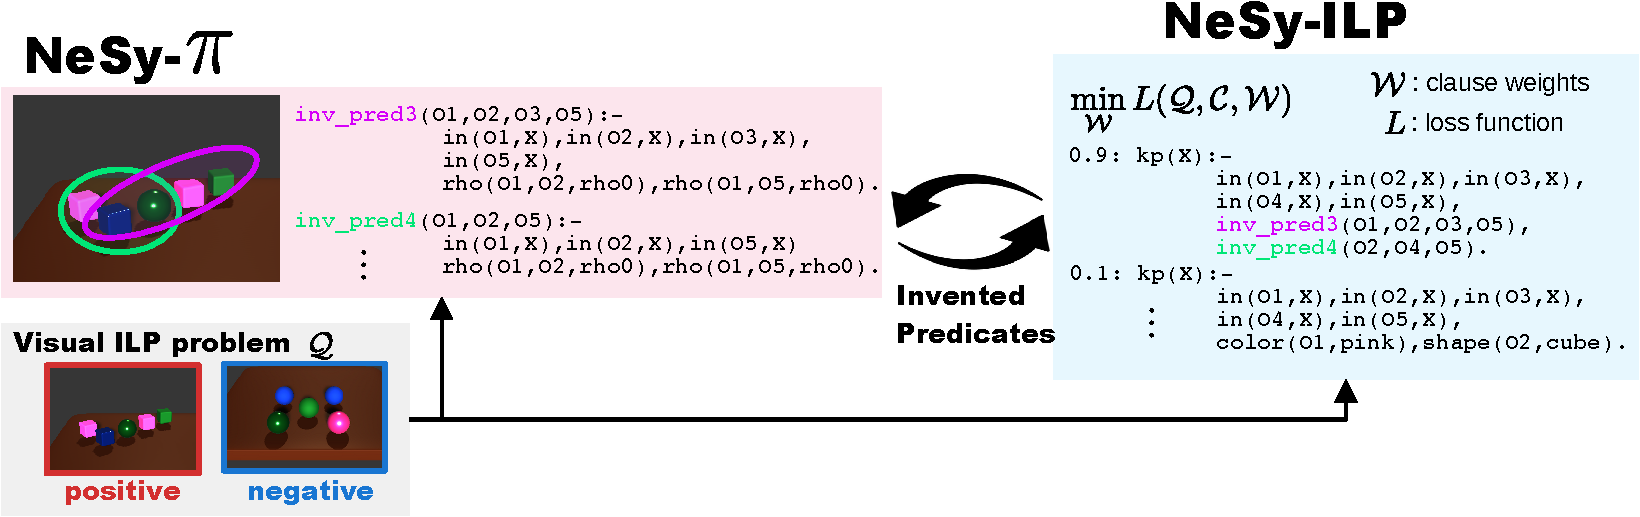
\includegraphics[width=\linewidth]{img/nesypi.pdf}
		\caption{\textbf{NeSy-$\pi$ architecture.} NeSy-$\pi$ invents relational concepts given visual scenes. The invented predicates are fed into a NeSy-ILP solver to learn classification rules. NeSy-ILP solver generates candidates of rules using given predicates, performs differentiable reasoning using weighted clauses, and optimize the clause weights by gradient descent. To this end, the classification rules can be composed efficiently using the invented predicates. (Best viewed in color) \hk{first draft, should be improved} \hk{do we have the opposite arrow: NeSy-ILP -> NeSy-pi in the system?}
			\js{Nope, the arrow that can point to NeSy-PI is from extended clauses, clauses are evaluated by NSFR first, then mapped to four score map, then good ones clustered as new predicates.}
		}
		\label{fig:nesypi}
	\end{figure}
	
	%% motivation of this paper, and point out the importance of this paper
	To this end, we propose Neural-Symbolic Predicate Invention (NeSy-$\pi$), a predicate invention pipeline that can invent relational concepts given visual scenes by finding rules defining them using primitive predicates.
	NeSy-$\pi$ can be integrated with existing NeSy-ILP systems so that they gain rich vocabulary to compose efficient solutions. \dd{till here}
	%and concatenate it with existing NeSy-ILP system, so that some high level concepts are not necessarily given from reasoning language directly. But they can be invented as needed during training. 
	%It can improve the system independence on human experts and also improves the generalization of AI models for adapting unseen tasks. 
	NeSy-$\pi$ reduces the amount of priors to be given by human experts or pre-training of neural modules, and thus extends the applicability of NeSy-ILP systems.
	NeSy-$\pi$ discovers predicates describing attributes of objects and their spatial relationships in visual scenes.
	We propose NeSy-$\pi$, a neural-symbolic PI approach, based on \textit{clustering} and \textit{extension} of relational concepts, which is able to reasoning visual scenes without background knowledge. The knowledge can be summarized from scenes. It evaluates the clauses based on its characteristics of necessity and sufficiency. The procedure is repeated iteration by iteration, until the target clauses are found. We tested our approach on both 2D and 3D image patterns.
	For example, the concepts like left, right, nearby supposed to be invented as new predicates during the training if any of them are needed to represent the target pattern in the positive images.  This map both considers the distance and directions of the latent relation objects. 
	We designed an evaluation function based on the characteristics of necessity and sufficiency of the clause, which can scoring the searched clauses and keep the promising ones for further extension.
	%% works of this paper and its contribution
	%In this paper, we mainly focus on object property and their spatial relationships comparison. In order to using a single language to cover two objects spatial relations as many as possible, we designed an area division map called \textit{target map} as shown in figure \ref{fig:8-area}, they are mapped to neural predicates as consider as basic predicates for PI model. As we shown in the experiment, the concepts like left, right, nearby supposed to be invented as new predicates during the training if any of them are needed to represent the target pattern in the positive images.  This map both considers the distance and directions of the latent relation objects. 
	
	%The target clause is searched in a top-bottom way, i.e. we start from most general rules and extend the rules by adding predicates as constraints. The size of searching domain for the target clause is growth exponentially over its length, which make the evaluation very time consuming. Since a naive pruning strategy can eliminate the global optimal clause. 
	
	
	
	%Comparing to existing approaches, our approach has following contributions
	Overall, we make the following important contributions:
	
	% \begin{itemize}
		%\item We proposed a predicate invention approach for neural-symbolic ILP system.
		\textbf{(1)} We propose NeSy-$\pi$, which is a NeSy predicate invention framework compatible with NeSy ILP systems. NeSy-$\pi$ extends NeSy ILP systems by providing the capability to enrich their vocabularies by learning from data.
		\textbf{(2)} We develop $3$D Kandinsky Patterns, which are user-friendly 3D image-generation systems according to abstract patterns on attributes and relations of objects. It extends Kandisnky patterns to the 3D world, and it achieves faster generation than other environments, \eg CLEVR~\cite{}.
		% 	\item A formalized way to efficiently evaluate the clauses in visual scenes, which can be further used for pruning strategy.
		\textbf{(3)} Complex shapes \dd{extend}
		\textbf{(4)} We discussed about \textit{when} and \textit{how} to invent new predicates based on \textit{necessary} and \textit{sufficient} judgment factors. \dd{rewrite}
		% 	\item The provide an implementation of this approach.
	%\end{itemize}
	%\hk{Contributions are about: What are we providing to the nesy community? What will they gain by our paper?}
	
	\section{First-order Logic and Inductive Logic Programming}
	
	{\bf First-Order Logic (FOL).}
	A {\it Language} $\mathcal{L}$ is a tuple $(\mathcal{P}, \mathcal{A}, \mathcal{F}, \mathcal{V})$,
	where $\mathcal{P}$ is a set of predicates, $\mathcal{A}$ is a set of constants, $\mathcal{F}$ is a set of function symbols (functors), and $\mathcal{V}$ is a set of variables.
	A {\it term} is a constant, a variable, or a term that consists of a functor.
	A {\it ground term} is a term with no variables.
	We denote $n$-ary predicate ${\tt p}$ by ${\tt p}/n$.
	An {\it atom} is a formula ${\tt p(t_1, \ldots, t_n) }$, where ${\tt p}$ is an $n$-ary predicate symbol and ${\tt t_1, \ldots, t_n}$ are terms.
	A {\it ground atom} or simply a {\it fact} is an atom with no variables.
	A {\it literal} is an atom or its negation.
	A {\it positive literal} is just an atom. 
	A {\it negative literal} is the negation of an atom.
	A {\it clause} is a finite disjunction ($\lor$) of literals. 
	A {\it ground clause} is a clause with no variables.
	A {\it definite clause} is a clause with exactly one positive literal.
	If  $A, B_1, \ldots, B_n$ are atoms, then $ A \lor \lnot B_1 \lor \ldots \lor \lnot B_n$ is a definite clause.
	We write definite clauses in the form of $A~\mbox{:-}~B_1,\ldots,B_n$.
	Atom $A$ is called the {\it head}, and set of negative atoms $\{B_1, \ldots, B_n\}$ is called the {\it body}.
	We call definite clauses as clauses for simplicity in this paper.
	We denote $\mathit{true}$ as $\top$ and $\mathit{false}$ as $\bot$.
	Substitution $\theta = \{\tt X_1 = t_1, ..., X_n = t_n\}$ is an assignment of term ${\tt t_i}$ to variable ${\tt X_i}$. An application of substitution $\theta$ to atom $A$ is written as $A \theta$. An atom is an atomic \emph{formula}. For formula $F$ and $G$, $\lnot F$, $F \land G$, and $F \lor G$ are also formulas.
	\emph{Interpretation} of language $\mathcal{L}$ is a tuple $(\mathcal{D}, \mathcal{I}_\mathcal{A}, \mathcal{I}_\mathcal{F}, \mathcal{I}_\mathcal{P})$, 
	where $\mathcal{D}$ is the  domain, $\mathcal{I}_\mathcal{A}$ is the assignments of an element in $\mathcal{D}$ for each constant ${\tt a} \in \mathcal{A}$,
	$\mathcal{I}_\mathcal{F}$ is the assignments of a function from $\mathcal{D}^n$ to $\mathcal{D}$ for each $n$-ary function symbol ${\tt f} \in \mathcal{F}$, 
	and $\mathcal{I}_\mathcal{P}$ is the assignments of a function from $\mathcal{D}^n$ to $\{ \top, \bot \}$ for each $n$-ary predicate ${\tt p} \in \mathcal{P}$.
	For language $\mathcal{L}$ and formala $X$, an interpretation $\mathcal{I}$ is a \emph{model} if the truth value of $X$ w.r.t $\mathcal{I}$ is true.
	Formula $X$ is a \emph{logical consequence} or \emph{logical entailment} of a set of formulas $\mathcal{H}$, denoted $\mathcal{H} \models X$, if, $\mathcal{I}$ is a model for $\mathcal{H}$ implies that $\mathcal{I}$ is a model for $X$ for every interpretation $\mathcal{I}$ of $\mathcal{L}$.
	
	
	\textbf{Inductive Logic Programming.}
	ILP problem $\mathcal{Q}$ is tuple $(\mathcal{E}^+, \mathcal{E}^-, \mathcal{B}, \mathcal{L})$, where
	$\mathcal{E}^+$ is a set of positive examples, $\mathcal{E}^-$ is a set of negative examples, $\mathcal{B}$ is background knowledge, 
	and $\mathcal{L}$ is a language. We assume that the examples and the background knowledge are ground atoms.
	The solution to an ILP problem is a set of definite clauses $\mathcal{H} \subseteq \mathcal{L}$
	that satisfies the following conditions:
	\begin{itemize}
		\item $\forall A \in \mathcal{E}^+ ~ \mathcal{H} \cup \mathcal{B}  \models A$.
		\item $\forall A \in \mathcal{E}^-  ~\mathcal{H} \cup \mathcal{B} \not \models A.$
	\end{itemize}
	Typically the search algorithm starts from general clauses. If the current clauses are too general (strong), i.e., they entail too many negative examples, then the solver incrementally specifies (weakens) them.
	This weakening operation is called a {\it refinement}, which is one of the essential tools for ILP.
	
	
	\textbf{Ne-Sy Inductive Logic Programming.} We address the ILP problem in visual scenes, which is called \emph{visual ILP problem}, where each example is given as an image containing several objects.
	The classification pattern is defined on high-level concepts such as attributes and relations of objects.
	
	$\alpha$ILP learns differentiable logic programs that describe complex visual scenes.
	We basically follow the differentiable ILP setting~\cite{Evans2018,Shindo21}, where an ILP problem is formulated as an optimization problem that has the following general form:
	\textbf{(Step 1)} Generate candidates of clauses $\mathcal{C}$ given language $\mathcal{L}$, and assign clause weights $\mathcal{W}$ to $\mathcal{C}$. 
	\textbf{(Step 2)} Optimize the clause weights $\mathcal{W}$ to minimize a classification loss, \ie  $\mathcal{W}^*= \min_\mathcal{W} \mathit{loss}(\mathcal{Q}, \mathcal{C}, \mathcal{W}),$
	%\begin{align}
	%    \mathcal{C} &= \texttt{clause\_generation}(\mathcal{L})  \\
	%    
	%\end{align}
	where $\mathcal{Q}$ is an ILP problem, $\mathcal{C}$ is a set of candidates of clauses, $\mathcal{W}$ is a set of weights for clauses, and $\mathit{loss}$ is a loss function that returns a penalty when training constraints are violated.
	We note that we solve visual ILP problems, where each positive and negative example is an image containing several objects.
	$\alpha$ILP~\cite{Shindo2023alphailp} is a NeSy-ILP system which handles complex visual scenes, which learns to represent scenes as logic programs. Intuitively, logical atoms correspond to objects, attributes, and relations, and clauses encode high-level scene information. $\alpha$ILP has an end-to-end reasoning architecture from visual inputs and learns differentiable logic programs by gradient descent.
	
	\section{Neuro-Symbolic Predicate Invention: NeSy-$ \pi $}
	We propose NeSy-$\pi$, which invenvts new predicates for NeSy-ILP solver from dataset.
	Given dataset $\mathcal{D}$, NeSy-$\pi$ aims to enrich language $\mathcal{L}$ by inventing new predicates that lead NeSy-ILP systems to generate better set of clause $\mathcal{C}$. The workflow of NeSy-$\pi$ is shown in Fig.~\ref{fig:nesypi_flow}.
	Given language $\mathcal{L}$ and dataset $\mathcal{D}$, NeSy-$\pi$ produces enriched language $\mathcal{L}^*$ by  iterating the following \emph{two} steps:  \emph{evaluate existing predicates} and \emph{invent new predicates}. 
	We describe each step in detail.
	\begin{figure}
		\centering
		\includegraphics[width=.7\linewidth]{img/nesypi_flow.pdf}
		\caption{\textbf{The workflow of NeSy-$\pi$.} Given language $\mathcal{L}$ and dataset $\mathcal{D}$, NeSy-$\pi$ produces enriched language $\mathcal{L}^*$ by inventing new predicates. $\mathcal{L}$ contains premitive predicates, and $\mathcal{D}$ consists of pairs of positive and negative visual scenes. (Best viewed in color) \hk{maybe in wrapfigure} }
		\label{fig:nesypi_flow}
	\end{figure}
	
	\textbf{Predicate Evaluation.}
	We evaluate each predicate to select to compose new predicates. 
	Promising predicates are those that can compose a clause entailing many positive examples but no negative examples.
	We develop \emph{two} evaluation metrics for predicates in NeSy-ILP systems, which we call \emph{necessity} and \emph{sufficiency}. Intuitively, \emph{necessary} predicates are those that are useful to compose clauses that do not entail negative examples, and \emph{sufficient} predicates are those that entail many positive examples.
	NeSy-$\pi$ computes these metrics efficiently by mapping the training pairs to a 2D Euclidean space, as shown in Fig.~\ref{fig:score}.
	
	NeSy-$\pi$ maps each training pair $(x_i^+, x_i^-) \in \mathcal{D}$, to a point in a 2D Euclidean scoring space $(r_\mathcal{C}(x_i^+), r_\mathcal{C}(x_i^-)) \in [0,1]^2$, where $r_\mathcal{C}$ is a reasoning function given clauses $\mathcal{C}$.
	$r_\mathcal{C}{x_i^+}$ represents the \emph{true positive} score, which is a probability for a positve example to be classified positive.
	$r_\mathcal{C}{x_i^-}$ represents the \emph{false positive} score, which is a probability for a negative example to be classified positive.
	On the scoring space, the \emph{necessity} of predicates are measured as
	\begin{align}
		f_\mathit{ness}(\mathcal{C}, \mathcal{D}) = |\{(x_i^+, x_i^-) ~|~  (x_i^+, x_i^-) \in \mathcal{D} ~ \land ~  r_\mathcal{C}(x_i^-) < \theta^-  \}|,
	\end{align}
	where $\theta^- \in [0,1]$ is a threshold for the \emph{false positive} score.
	The \emph{sufficiency} of predicates are measured as:
	\begin{align}
		f_\mathit{ness}(\mathcal{C}, \mathcal{D}) = |\{(x_i^+, x_i^-) ~|~  (x_i^+, x_i^-) \in \mathcal{D} ~ \land ~  r_\mathcal{C}(x_i^+) > \theta^+  \}|,
	\end{align}
	where $\theta^+ \in [0,1]$ is a threshold for the \emph{true positive} score.
	
	\textbf{Predicate Invention.}
	NeSy-$\pi$ invents new predicates using the scores over predicates. \hk{continue}
	
	
	
	%\textbf{Problem Statement.}
	%\begin{align}
	%    \mathcal{L}^* &= \mathtt{invent\_predicates}(\mathcal{L}, \mathcal{D})\\
	%    \mathcal{C} &= \texttt{clause\_generation}(\mathcal{L}^*)  \\
	%    \mathcal{W}^* &= \min_\mathcal{W} \mathit{loss}(\mathcal{Q}, \mathcal{C}, \mathcal{W}),
	%\end{align}
	
	%The target of inductive logic programming is to find a target clause $ P $ for the positive patterns $Q$, such that the clause $ P $ describes some logical relations that exist and only exist in the positive patterns. 
	%Thus the target clause $ P $ is sufficient and necessary for the positive patterns $ Q $.
	%\[ P\Leftrightarrow Q \]
	
	%%
	%TODO: tell the way of clause generation
	%We prepare equal number of positive and negative images for evaluation, thus all the images can be paired from two groups. We define PN pair as a pair of positive and negative images. 
	%A new generated clause is evaluated on all the PN pairs. Evaluation on each pair getting two values, one from positive and one from negative. 
	% We can take negative value as x axis, positive value as y axis and draw all the evaluation result on a coordinate system. Thus each PN pair corresponds a point. We observed these points are only appears in the four clusters in the coordinate system( as show in figure \ref{fig:pn-pair} middle.), thus we fuzzy these points to only four areas, each take one cluster. Thus for these two values, we only have $ 2^2=4 $ different combinations. We named it as \textit{four score map}.
	
	\if0
	\begin{figure*}[t]
		\centering
		\begin{minipage}{\textwidth}
			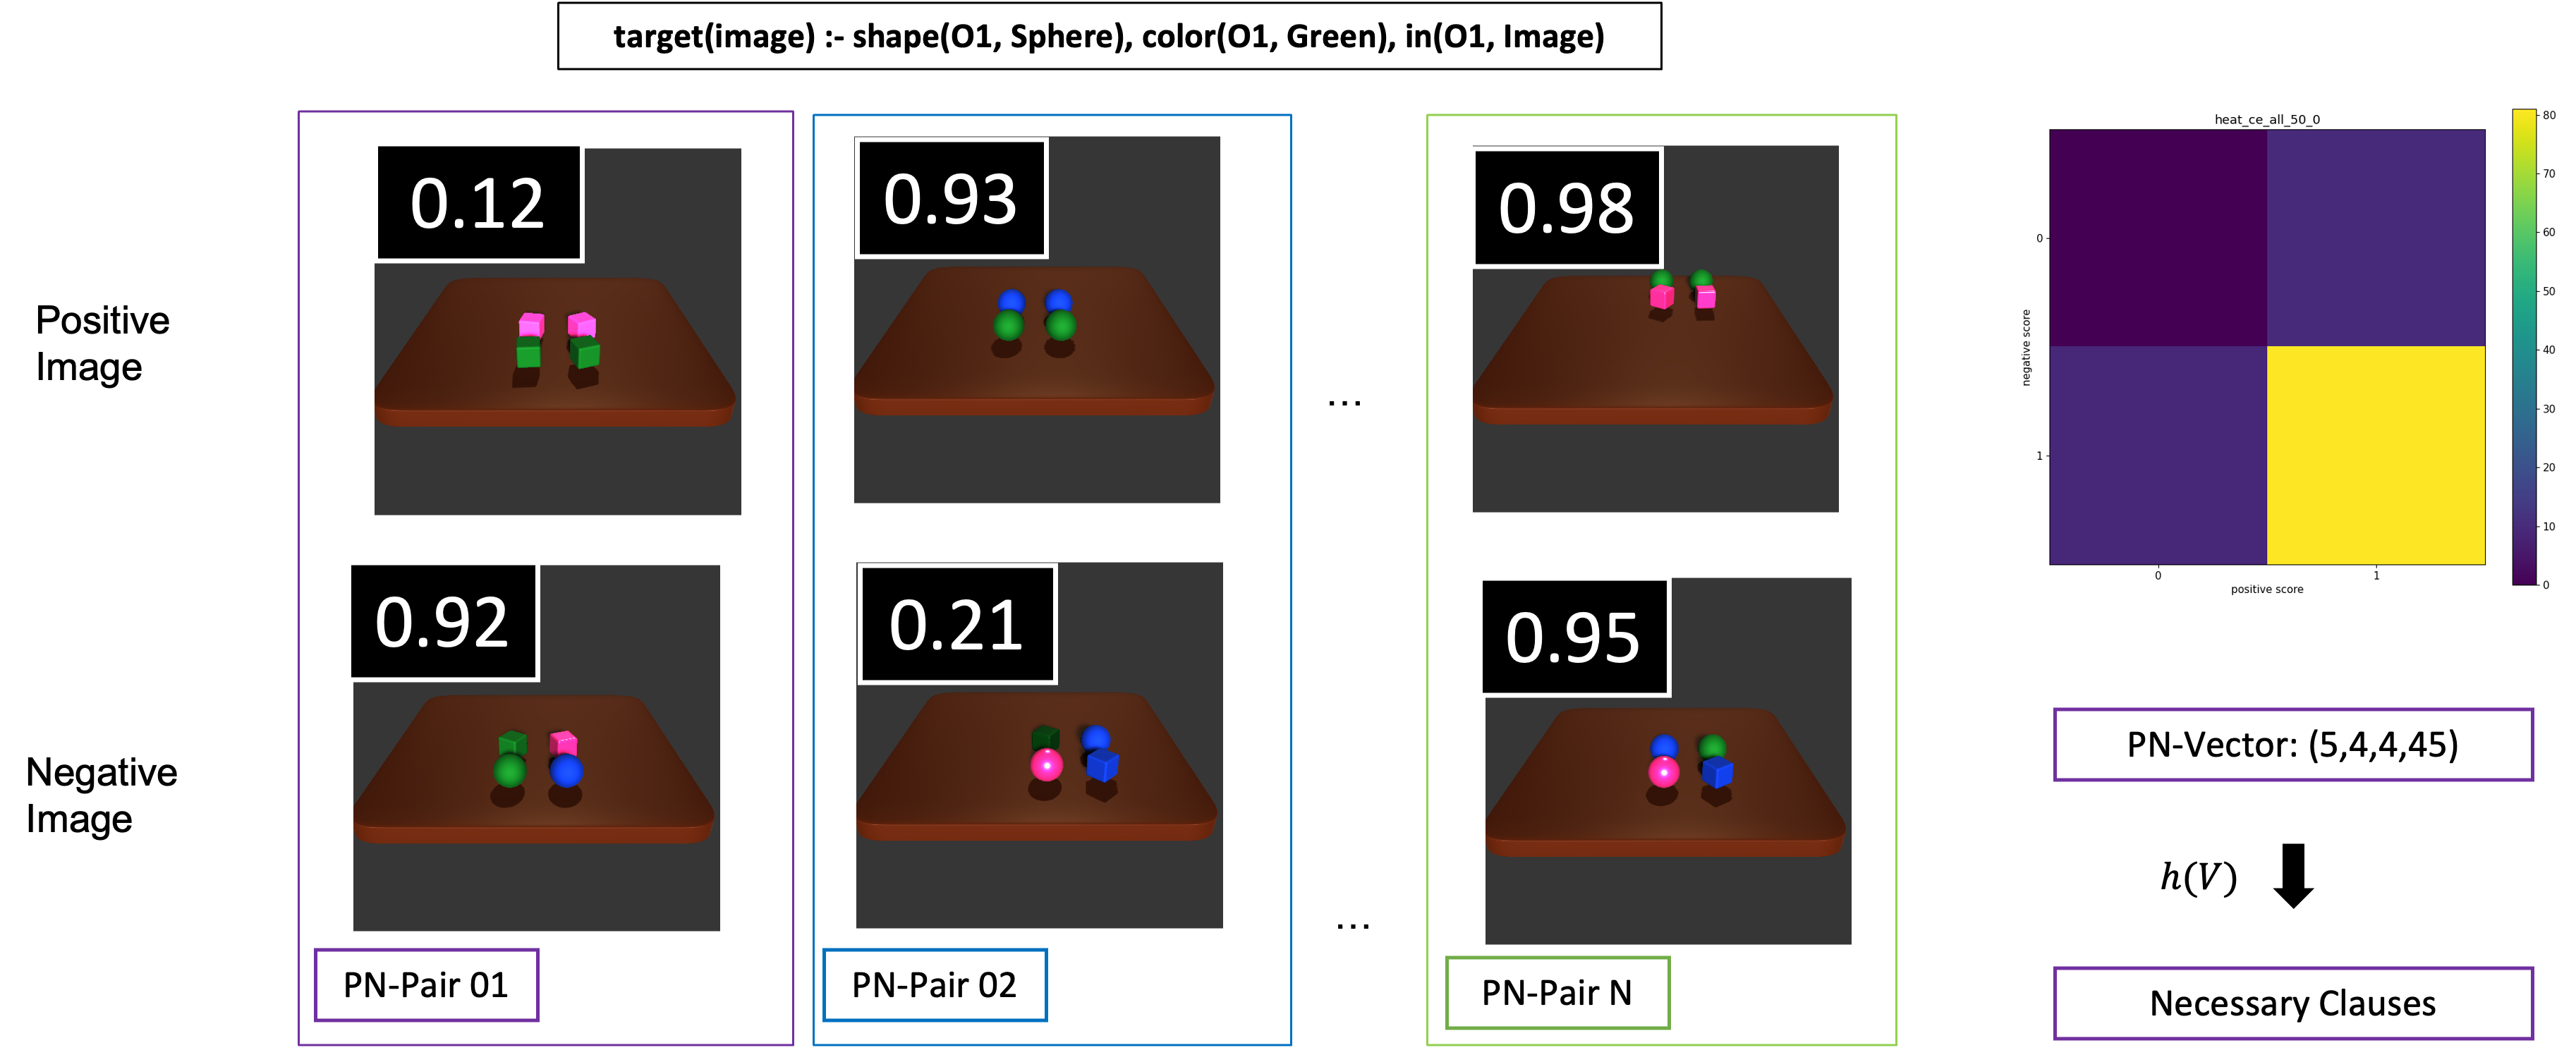
\includegraphics[width=\linewidth]{img/four_zone_explain.png} 
			\caption{\textbf{Left}: PN pairs. \textbf{Middle}: PN pair scores on coordinate system. The points are clustered in four corners. These scores are evaluated by NSFR. \textbf{Right:}Four Score Map. The four score map illustrates the result of 4 kinds of evaluation on one clause, i.e. high positive-high negative, high positive-low negative, low positive-high negative, low positive-low negative. }
			\label{fig:pn-pair}
		\end{minipage}
	\end{figure*}
	\fi
	
	\begin{figure}[t]
		\centering
		\includegraphics[width=\linewidth]{img/nesypi_score.pdf}
		\caption{\textbf{Scoring strategy in NeSy-$\pi$.} NeSy-$\pi$ takes an input as a pair of positive and negative example $(x_i^+, x_i^-)$, applies the reasoning function $r_\mathcal{C}$ using clauses $\mathcal{C}$ to compute a scalar value for each (left). The computed pair of scalar values are casted to a 2D Euclidean scoring space. $f_\mathit{ness}$ quantifies the necessity of clauses $\mathcal{C}$ for dataset $\mathcal{D}$, \ie it counts the number of training pairs in $\mathcal{D}$ whose negative example is not entailed by $\mathcal{C}$, and $f_\mathit{suff}$ quantifies the sufficiency of clauses $\mathcal{C}$ for dataset $\mathcal{D}$, \ie it counts the number of training pairs in $\mathcal{D}$ whose positive example is entailed by $\mathcal{C}$  (right). \hk{first draft, need to be improved} }
		\label{fig:score}
	\end{figure}
	
	
	
	%A \textbf{four score map} fuzzy the evaluation result on an image to positive 1 and negative 0, map the positive image result and negative image result to four areas, namely $ (0,0), (0,1), (1,0) $ and $ (1,1) $. We found that four score map has good description for sufficient and necessary conditions in logic.
	
	%Base on the scoring areas of the predicates, we can classify them into several groups. Let $ N $ denotes the number of PN pairs.
	
	%\hk{change to 2 metrics}
	%\begin{definition}[Sufficient and Necessary Clause]
	%	Scores on $ (0,1) $ only, i.e. $ s_{01} =N$ They are sufficient and necessary for the target pattern.
	%\end{definition}
	
	%\begin{definition}[Necessary Clause]
	%	Scores on $ (0,1) $ and $ (1,1) $, i.e. $ s_{01} + s_{11} = N $. They are necessary for the target pattern. Note that they always true in the positive images, but also can be true in negative images.
	%\end{definition}
	
	%\begin{definition}[Sufficient Clause]
	%	Scores on $ (0,0) $ and $ (0,1) $, $ s_{00}+s_{01} = N $ and $ s_{01}>0 $. It induces directly some of positive patterns but can be failed on some other positive patterns. It never induces any negative patterns.
	%\end{definition}
	
	
	
	The key idea of these definitions is to provide an evaluation metric for searched clauses. Since it is impossible to consider all the clauses for rule searching, an efficient pruning strategy is necessary. Our pruning strategy is mainly based on the satisfaction of the clauses on these definitions. 
	The workflow of NeSy-$ \pi $ is shown in figure \ref{fig:nesy-pi-workflow.}. The system's work is basically to maintain a clause set $ \mathcal{C} $. We add promising clauses inside and remove the abandoned ones from it. We explain each state as follows
	\paragraph{Initial}
	The searching is started from here. The input is the most general clause, i.e. the one that only states the existence of objects in the scene. For a scene with at most 2 objects, the initial clause set is $ \mathcal{C} = \{\mathtt{target(X):-in(O1,X),in(O2,X).} \} $. Note that initial clause is a necessary clause since it is true on all the positive images.
	
	\paragraph{Extend}
	The input is either the initial clause set or the clauses set from pruning. For each clause in the set, we extend it with one predicate. Since there are many possible predicates to chose, any of them can be a promising one, thus we consider all the extension possibility into account. For example, to extend clause $ c $, if there are 10 predicates in the language, the number of extended clauses of $ c $ is up to 10, if all the extended clauses are consistent with itself.
	
	\paragraph{Evaluate}
	In order to find all the promising clauses, we evaluate all the extended new clauses or clustered clauses. For each evaluation unit, we evaluate it on the whole dataset and classify it based on its four score map.
	
	\paragraph{Pruning}
	Pruning is based on scores of each clause or clause cluster getting from evaluate state. A prune strategy is required in this step. In this paper, we select only top ranked necessary/sufficient clauses/clusters, the rests are pruned. 
	
	\paragraph{Cluster}
	The cluster is one step as preparation of high level concepts invention. 
	For example, if $ \mathtt{blue}, \mathtt{red} $  are the only appearing colors in all the scenes,  the concept $ \mathtt{two\_objs\_with\_same\_color} $ can be clustered by clauses 
	\begin{align*}
		\mathtt{two\_objs\_with\_same\_color(X)}&\mathtt{\texttt{:-}in(O1,X),in(O2,X),color(O1,Blue),color(O2,blue).}\\ \mathtt{two\_objs\_with\_same\_color(X)}&\mathtt{\texttt{:-}in(O1,X),in(O2,X),color(O1,Red),color(O2,red).}
	\end{align*}
	After pruning, if the max iteration of clause extension is exceed, the system will cluster the clauses. The input is clause set $ \mathcal{C} $. 
	We calculate all the subsets of $ \mathcal{C} $. Each subset is considered as one cluster. The number of clusters is up to $ 2^n $, where $ n=|\mathcal{C}| $ i.e. the size of clause set. Since it grows exponentially, for a large $ n $, we cannot evaluate all the subset. In order to improve the computation efficiency, the size of subset can be constrained with a threshold, to control the maximum size of the subset.
	
	\paragraph{Inventing}
	The input of inventing state is the set of clause clusters. Each cluster is considered as a new predicate, where its body is the clause clusters. After invention, the new predicates update the language and the system goes to initial state again.
	
	\paragraph{Finish} 
	The system finish the rule searching if any sufficient and necessary predicate or clause is found or failed by exceeding the maximum iterations.
	
	
	
	\section{Experimental Evaluation}
	% \hk{List questions to be answered?} \dd{Yep}
	We aim to answer the following questions:
	\begin{enumerate}
		\item[\textbf{Q1:}] Does NeSy-$\pi$ invent predicates from complex visual scenes for NeSy ILP systems to reduce required background knowledge?
		\item[\textbf{Q2:}] Is NeSy-$\pi$ computationally efficient?
		\item[\textbf{Q3:}] Can 3D Kandinsky patterns provide efficient evaluations for NeSy-ILP systems?
	\end{enumerate}
	
	\paragraph{A1}: We designed four kinds of visual scenes for 2D KP and 3D KP respectively, as shown in Fig. \ref{fig:3DKP-patterns} and Appendix . To solve such patterns, NeSy-ILP system without PI module requires several background knowledge and related predicates to help the system reasoning about the final rules. For example, some scenes require the knowledge $ \mathtt{one\_pair(A,B)} $ like \textit{three same} and \textit{two pairs}. In NeSy-ILP, such pattern can be solved by providing following BK
	\begin{lstlisting}[language=Prolog,  style=Prolog-pygsty]
one_pair(A,B):-same_color_pair(A,B),same_shape_pair(A,B),in(A,X),in(B,X).
same_shape_pair(A,B):-shape(A,Sq),shape(B,Sq),in(A,X),in(B,X).
same_shape_pair(A,B):-shape(A,Cir),shape(B,Cir),in(A,X),in(B,X).	
same_color_pair(A,B):-color(A,Red),color(B,Red),in(A,X),in(B,X).
same_color_pair(A,B):-color(A,Blue),color(B,Blue),in(A,X),in(B,X).
	\end{lstlisting}
	It requires 5 background clauses to explain the concept $ \mathtt{one\_pair} $, and the 6 predicates $ \mathtt{one\_pair(A,B), same\_shape\_pair(A,B), same\_color\_pair(A,B), shape(A,Y), color(A,Z) } ,$ $  \mathtt{in(A,X)} $ to construct the clauses.
	In NeSy-$ \pi $, such kind of background clauses are not provided but learned by system. The concepts are invented  as new predicates. A possible solution from our system can be learned as follows
	\begin{lstlisting}[language=Prolog,  style=Prolog-pygsty]
target(A,B):-in(O1,X),in(O2,X),inv_pred2(O1,O2).
inv_pred1(O1,O2):-color(O1,Blue),color(O2,Blue),in(O1,X),in(O2,X).
inv_pred1(O1,O2):-color(O1,Red),color(O2,Red),in(O1,X),in(O2,X).
inv_pred2(O1,O2):-in(O1,X),in(O2,X),inv_pred1(O1,O2),shape(O1,Cir),shape(O2,Cir).
inv_pred2(O1,O2):-in(O1,X),in(O2,X),inv_pred1i(O1,O2),shape(O1,Sq),shape(O2,Sq).
	\end{lstlisting}
	In this example, only 3 predicates ($\mathtt{shape(A,Y), color(A,Z) , in(A,X)} $) are given beforehand as neural predicates and no further clauses is required, which is significantly reduce the knowledge reliance. In all the patterns in our experiments, we give no such BK clauses and provide in total 6 neural predicates for reasoning, where each predicate returns the confidence of its truth. 
	$ \mathtt{in/2/O,X} $: the object $\mathtt{O}$ exists in the image $\mathtt{X}$. 
	$ \mathtt{shape/2/O,S} $: the object $\mathtt{O}$ has shape $\mathtt{S}$. 
	$\mathtt{color/2/O,C}$: the object $\mathtt{O}$ has color $\mathtt{C}$.
	$\mathtt{phi/2/O_1,O_2, \phi}$: the object $\mathtt{O_2}$ is located in the direction $\phi$ of $\mathtt{O_1}$ as calculated in polar coordinate system..
	$\mathtt{rho/2/O_1,O_2, \rho}$: the distance between object $\mathtt{O_2}$ and $\mathtt{O_1}$ is around $\rho$.
	Besides, we provide the constants as the arguments for the given predicates. 
	
	\paragraph{A2}:
	Computation efficient...argue with time, prune strategy.
	ILP can be faster, since it has less predicates, but also can be failed, it is not efficient if keep search until found the target clause.
	
	
	\paragraph{A3}:
	Efficient evaluation? 
	evaluate clauses, it can indeed found the target clause, thus it is efficient.
	
	To solve 2D Kandinsky Patterns, we provide following constants as background knowledge, 
	shape: $\mathtt{square/triangle/circle}$; 
	color: $\mathtt{red/yellow/blue}$; 
	distance: from 0 to the maximum distance (the image width), we divide it to 8 levels, denote by $\mathtt{\rho_1/.../\rho_8}$, where $\rho_1 $ denote the distance within 0 pixel, $\rho_8$ corresponds the distance equal to the width of the image, others denote something in between; 
	direction: similar to distance, the direction is represented by 8 predicates $\phi_1/.../\phi_8 $ where each one corresponds $360/8=45^\circ$ of direction. \hk{We need a visual explanation for this}
	No further information is given, such as different color, different shape, etc. Fig. \ref{fig:kandinsky-patterns} shows some of the patterns in 2DKP. 
	
	\begin{figure}[t]%[!htb]
		\centering
		\includegraphics[width=0.7\textwidth]{img/pos_pred_explain.pdf}
		\caption{Position neural predicates based on polar coordinate system. \hk{texts should be bigger}}
		\label{fig:pos-pred-explain}
	\end{figure}
	
	To solve 3D Kandinsky Patterns, we provide following constants as background knowledge, 
	shape: $\mathtt{sphere/cube}$; 
	color: $\mathtt{pink/green/blue}$; 
	distance: all the positions of 3D objects are normalized. 8 distance predicates  are used to represent 8 levels of distance evenly;
	direction: we assume all the object place on a flat surface with similar height, thus the direction between two objects can be represented by two values only. We divide the direction into 8 levels evenly where each one corresponds $45^\circ$ of directions.
	\ref{fig:kandinsky-patterns} shows some of the patterns in 3DKP.
	The learning result on each patterns in Kandinsky pattern is shown in table \ref{tab:pi-result}.
	Fig.~\ref{fig:rules_cross_3DKP} shows the learned clause and invented predicates of \textit{cross} pattern in 3DKP.
	
	
	
	
	\begin{figure}[!htb]
		\centering
		\subfigure[Three Same]{
\includegraphics[width=0.24\textwidth]{img/3DKP/3_same.png}} 
		\subfigure[Two Pairs]{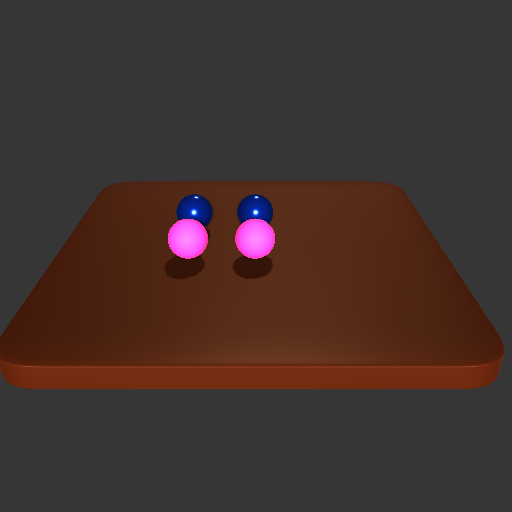
\includegraphics[width=0.24\textwidth]{img/3DKP/two_pairs.png}} 
		\subfigure[Shape in Shape]{\includegraphics[width=0.24\textwidth]{img/3DKP/shape_in_shape_true_2.png}} 
		\subfigure[Check Mark]{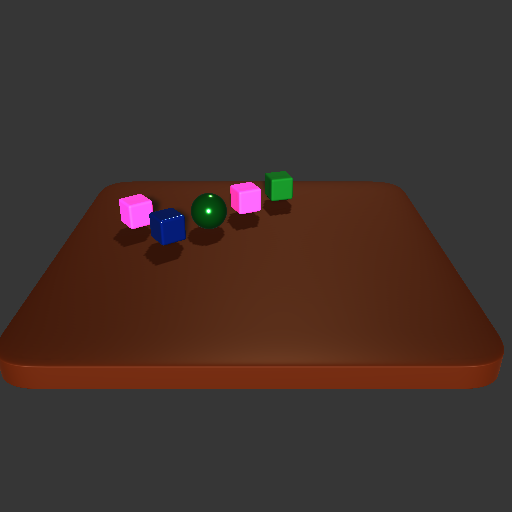
\includegraphics[width=0.24\textwidth]{img/3DKP/check_mark.png}} 
		\caption{3D Kandinsky Patterns. 
			\textbf{Three Same}: This pattern always have 3 objects inside, three of them has same color and same shape. 
			\textbf{Two Pairs}: This pattern always have 4 objects inside, two of them has same color and same shape. The other two also have same color and same shape.
			\textbf{Shape in Shape}: this pattern always have 4 objects with same shape inside, if they are cubes, their positions form a shape of square; if they are spheres, their positions form a shape of triangle.
			\textbf{Check Mark}: this pattern always have 5 objects, the position of 5 objects consists of an outline of a check mark.}
		\label{fig:3DKP-patterns}
	\end{figure}
	
	
	
	%\begin{lstlisting}[language=Prolog, mathescape]
	\begin{figure}[t]
		\centering
		\begin{lstlisting}[language=Prolog,  style=Prolog-pygsty]
target(X):-in(O1,X),in(O2,X),in(O3,X),in(O4,X),in(O5,X),
inv_pred15(O1,O2,O3,O4,O5).

inv_pred15(O1,O2,O3,O4,O5):-in(O1,X),in(O2,X),in(O3,X),in(O4,X),in(O5,X),
inv_pred6(O2,O3,O4,O5),shape(O1,cube),shape(O2,cube),shape(O3,cube).

inv_pred15(O1,O2,O3,O4,O5):-in(O1,X),in(O2,X),in(O3,X),in(O4,X),in(O5,X),
inv_pred6(O2,O3,O4,O5),shape(O1,sphere),shape(O2,sphere),shape(O3,sphere).

inv_pred6(O1,O3,O4,O5):-in(O1,X),in(O3,X),in(O4,X),in(O5,X),
inv_pred3(O1,O3,O4,O5),phi(O3,O5,phi6),rho(O3,O5,rho1).

inv_pred3(O2,O3,O4,O5):-in(O2,X),in(O3,X),in(O4,X),in(O5,X), rho(O2,O5,rho2),
rho(O3,O4,rho2).
		\end{lstlisting}
		\label{fig:rules_cross_3DKP}
		\caption{Learned rules by NeSy-$\pi$ on Cross pattern in 3D Kandinsky Pattern scenes.}
	\end{figure}
	
	

\begin{table}
	\centering
	\begin{tabular}{c|c|c|c|c|c|c|c|c|c|c}
		\hline
		\toprule
		\multirow{2}*{Dataset} & \multirow{2}*{Patterns} &\multirow{2}*{\# obj} &  \multicolumn{2}{c|}{Iter.} &\multicolumn{2}{c|}{Time} & \multicolumn{2}{c|}{Accuracy} & \multicolumn{2}{c}{\# Preds} \\
		\cline{4-11}
		& & & $\alpha$ & $ \pi $ & $ \alpha$ & $ \pi $ &$ \alpha$ & $ \pi $&$ \alpha$ & $ \pi $\\
		\hline
		\multirow{4}*{2D KP} &
		Red Triangle &2	& 5 & 5 	&   9.18m & 5.28m &  0.83 & 1.0 & 16	   & 16 (+2)            \\
		&Two Pairs   & 4	& 5	& 4 &	 0.37m	& 8.91m & 0.57 & 1.0 & 4	& 	4 (+5)        \\
		&Check Mark & 5	& 5	& 6 &	 &  10.32m & & 1.0& 	&  	     \\
		&Cross Mark &5	&	& &	 	& & & & 	&  	       \\
		\hline
		\multirow{4}*{3D KP} &
		Same &  3 & 5 & 3	& 0.91m   &0.81m &  0.55 & 1.0 & 		  4  &       4 (+3)      \\
		&Two Pairs  & 4 & 5 & 3 & 	 0.46m	& 3.62m  & 0.62 & 1.0 & 4	& 4 (+5)  \\
		&Shape of Shape & 4 & 4 & 2  &	 14.69m	& 4.76m &  0.79 & 1.0 & 11 	& 	11 (+2)        \\
		&Check  Mark & 5 & 4 & 2  & 19.36m  & 19.28m & 0.87 & 1.0 &  12	& 	12 (+1)  \\
		\bottomrule
	\end{tabular}
	\caption{Experiment result on 2D Kandinsky Patterns and 3D Kandinsky Patterns. The dataset of each experiment has 64 PN pairs. $\alpha$ and $ \pi $ denote $\alpha$ILP system and NeSy-$\pi$ respectively. The numbers in the bracket of last column represent the number of invented predicates that are used in the target clauses.}
	\label{tab:pi-result}
\end{table}
	
	
\section{Related Work}
Inductive Logic Programming~\cite{Muggleton91,Muggleton95,Nienhuys97,Cropper20} has emerged at the intersection of machine learning and logic programming. Many ILP frameworks have been developed, e.g., FOIL~\cite{Quinlan90}, Progol~\cite{Muggleton95}, ILASP~\cite{ILASP}, Metagol~\cite{metagol,Cropper2019LearningHL}, and Popper~\cite{popper}.

Although predicate invention has been proposed since 1988 by \cite{MUGGLETON1988339}, it is always be considered as a major challenge. Most ILP system do not supports PI, including classic systems like Progol \cite{Muggleton1995InverseEA}, TILDE\cite{BLOCKEEL1998285} and modern system such as ATOM \cite{atom}, LFIT \cite{LFIT}.

Some works have been proposed for PI systems. 
Predicate Invention (PI) has been addressed~\cite{Stahl93PI,aAthakravi12PI,Cropper2019LearningHL,Hocquette20ijcaiPI,Kok2007StatisticalPI,KramerAustrian2007PI,Cropper_Morel_Muggleton_2020aaaiPI,Cropper21PI}. \hk{TODO: split}
However, none of these are focus on visual images and learning logical patterns existing in the visual scenes. 
\cite{pilff} is an approach for predicate invention, which generate constrains from inconsistent hypothesis and further be used for pruning all the similar clauses.
Several system \cite{Evans2018}, \cite{kaminski_eiter_inoue_2018} uses meta-rules as templates for new predicates invention. 
$ \alpha $ILP (citation?) supports visual image as input but require background knowledge during the reasoning.

	
	\section{Conclusion}
	
	In this paper, we proposed an approach for Neural-Symbolic Predicate Invention. NeSy-PI is able to find the new knowledge and summarize it as new predicates, thus it requires less background knowledge for reasoning.
	In our experiment, we show that our PI model can successfully find the target program given only basic neural perception results and relevant constants, no further background knowledge is required. We also show our efficient prune strategy for predicate searching, the searching result is acquired faster and still sound.
	
	\newpage
	\appendix
	\section{NeSy-$\pi$ algorithm}
	Alg. \ref{alg:pi} gives the pseudo code of the NeSy-$\pi$ system. 
	
	\begin{algorithm}
		\caption{NeSy-$ \pi $}\label{alg:pi}
		\begin{algorithmic}
			\State $C \gets C_0$
			\State $L \gets L_0$
			\While{ step < maxStep and not $succeed$}
			\For{$i\gets 1, ..., step $}
			\State $ C_{extended} \gets extend(C, L)$
			\State $S_c \gets  eval (C_{extended})$
			\State $C_{sn},C_{nc},C_{sc}, C_{uc} \gets  prune(C_{extended}, S_c)$
			\EndFor 
			\If {$C_{sn}.length()>0:$}
			\State $succeed \gets true$
			\State break
			\EndIf 
			\State $ C_{clu} \gets  cluster(C_{sn},C_{nc},C_{sc}, C_{uc} ) $
			\State $ S_{clu} \gets eval(C_{clu})$
			\State $ Clu_{sn}, Clu_{nc}, Clu_{sc}, Clu_{uc} \gets  prune(C_{clu}, S_{clu})$  
			\State $P_{new} \gets invent(L, Clu_{sn}, Clu_{nc}, Clu_{sc}, Clu_{uc})$
			\State $ L \gets update(L, P_{new})  $
			\State $step \gets step + 1$
			\EndWhile
			\State Train NSFR model
		\end{algorithmic}
	\end{algorithm}
	
	
	\section{Experiment details }
	\newpage
	\subsection{2D KP}
	
	Fig. \ref{fig:kandinsky-patterns} illustrates the 4 training patterns in 2D Kandinsky Dataset. 
	
	\begin{figure}[t]%[!htb]
		\centering
		\subfigure[True]{\includegraphics[width=0.24\textwidth]{img/kp/twopairs_true_1.png}} 
		\subfigure[True]{\includegraphics[width=0.24\textwidth]{img/kp/twopairs_true_2.png}} 
		\subfigure[False]{\includegraphics[width=0.24\textwidth]{img/kp/twopairs_false_1.png}} 
		\subfigure[False]{\includegraphics[width=0.24\textwidth]{img/kp/twopairs_false_2.png}} 
		
		\subfigure[True]{\includegraphics[width=0.24\textwidth]{img/kp/red_triangle_true_1.png}} 
		\subfigure[True]{\includegraphics[width=0.24\textwidth]{img/kp/red_triangle_true_2.png}} 
		\subfigure[False]{\includegraphics[width=0.24\textwidth]{img/kp/red_triangle_false_1.png}} 
		\subfigure[False]{\includegraphics[width=0.24\textwidth]{img/kp/red_triangle_false_2.png}} 
		
		\subfigure[True]{\includegraphics[width=0.24\textwidth]{img/kp/check_mark_true_2.png}} 
		\subfigure[True]{\includegraphics[width=0.24\textwidth]{img/kp/check_mark_true_1.png}} 
		\subfigure[False]{\includegraphics[width=0.24\textwidth]{img/kp/check_mark_false_1.png}} 
		\subfigure[False]{\includegraphics[width=0.24\textwidth]{img/kp/check_mark_false_2.png}} 
		
		\caption{Kandinsky Patterns. \textbf{Two Pairs}: This pattern always have 4 objects inside, two of them has same color and same shape, the other two has same shape and different color. \textbf{Red Triangle}: This pattern always have a red triangle, and another object with different color and different shape nearby, the rest 4 objects are random objects. \textbf{Check Mark}: the positions of 5 objects consists of an outline of check mark. It considers the symmetric pattern as positive as well, but the long side has to be in the right part. Otherwise it is false pattern. \textbf{Pattern 4}: \js{to be continue...}
		\label{fig:kandinsky-patterns}
	\end{figure}
	\newpage
	\subsection{3DKP}
	
	
	\begin{figure}[!htb]
		\centering
		\subfigure[True]{\includegraphics[width=0.24\textwidth]{img/3DKP/3_same_true_1.png}} 
		\subfigure[True]{\includegraphics[width=0.24\textwidth]{img/3DKP/3_same_true_2.png}} 
		\subfigure[False]{\includegraphics[width=0.24\textwidth]{img/3DKP/3_same_false_1.png}} 
		\subfigure[False]{\includegraphics[width=0.24\textwidth]{img/3DKP/3_same_false_2.png}} 
		
		\subfigure[True]{\includegraphics[width=0.24\textwidth]{img/3DKP/two_pairs_true_1.png}} 
		\subfigure[True]{\includegraphics[width=0.24\textwidth]{img/3DKP/two_pairs_true_2.png}} 
		\subfigure[False]{\includegraphics[width=0.24\textwidth]{img/3DKP/two_pairs_false_1.png}} 
		\subfigure[False]{\includegraphics[width=0.24\textwidth]{img/3DKP/two_pairs_false_2.png}} 
		
		\subfigure[True]{\includegraphics[width=0.24\textwidth]{img/3DKP/shape_in_shape_true_1.png}} 
		\subfigure[True]{\includegraphics[width=0.24\textwidth]{img/3DKP/shape_in_shape_true_2.png}} 
		\subfigure[False]{\includegraphics[width=0.24\textwidth]{img/3DKP/shape_in_shape_false_1.png}} 
		\subfigure[False]{\includegraphics[width=0.24\textwidth]{img/3DKP/shape_in_shape_false_2.png}} 
		
		
		\subfigure[True]{\includegraphics[width=0.24\textwidth]{img/3DKP/check_mark_true_1.png}} 
		\subfigure[True]{\includegraphics[width=0.24\textwidth]{img/3DKP/check_mark_true_2.png}} 
		\subfigure[False]{\includegraphics[width=0.24\textwidth]{img/3DKP/check_mark_false_1.png}} 
		\subfigure[False]{\includegraphics[width=0.24\textwidth]{img/3DKP/check_mark_false_2.png}} 
		\caption{Training examples in 3D Kandinsky Pattern Dataset. From top to bottom, 
			\textbf{Three Same}: Three objects with same color and same shape.
			\textbf{Two Pairs}: Four objects, two of them has same color and same shape, the other two has same color and same shape as well.
			\textbf{Shape in Shape}: Four objects with same shape. If all the objects are cubes, their positions forms a square shape. If all the objects are spheres, their position forms a triangle shape.
			\textbf{Check Mark}: Five objects form a check mark shape, the flipped or symmetry shapes are also considered as positive.}
		\label{fig:3DKP-patterns-full}
	\end{figure}
	
	%\begin{lstlisting}[language=Prolog, mathescape]
	\begin{figure}[t]
		\centering
		\begin{lstlisting}[language=Prolog,  style=Prolog-pygsty]
			
			(three same)
			kp(X):-in(O1,X),in(O2,X),in(O3,X),inv_pred2(O1,O2,O3).
			inv_pred2(O1,O2,O3):-color(O1,blue),color(O2,blue),color(O3,blue),
			in(O1,X),in(O2,X),in(O3,X),shape(O1,cube),shape(O2,cube),shape(O3,cube).
			inv_pred2(O1,O2,O3):-color(O1,blue),color(O2,blue),color(O3,blue),in(O1,X),
			in(O2,X),in(O3,X),shape(O1,sphere),shape(O2,sphere),shape(O3,sphere).
			inv_pred2(O1,O2,O3):-color(O1,green),color(O2,green),color(O3,green),in(O1,X),
			in(O2,X),in(O3,X),shape(O1,cube),shape(O2,cube),shape(O3,cube).
			inv_pred2(O1,O2,O3):-color(O1,green),color(O2,green),color(O3,green),in(O1,X),
			in(O2,X),in(O3,X),shape(O1,sphere),shape(O2,sphere),shape(O3,sphere).
			inv_pred2(O1,O2,O3):-color(O1,pink),color(O2,pink),color(O3,pink),in(O1,X),
			in(O2,X),in(O3,X),shape(O1,cube),shape(O2,cube),shape(O3,cube).
			inv_pred2(O1,O2,O3):-color(O1,pink),color(O2,pink),color(O3,pink),in(O1,X),
			in(O2,X),in(O3,X),shape(O1,sphere),shape(O2,sphere),shape(O3,sphere).
			
			
			(two pairs)
			kp(X):-in(O1,X),in(O2,X),in(O3,X),in(O4,X),inv_pred30(O1,O2,O3,O4),
			inv_pred7(O3,O4).
			inv_pred30(O1,O2,O3,O4):-in(O1,X),in(O2,X),in(O3,X),in(O4,X),inv_pred2(O1,O2),
			inv_pred2(O3,O4),inv_pred7(O1,O2).
			inv_pred7(O1,O2):-in(O1,X),in(O2,X),shape(O1,cube),shape(O2,cube).
			inv_pred7(O1,O2):-in(O1,X),in(O2,X),shape(O1,sphere),shape(O2,sphere).
			inv_pred2(O1,O2):-color(O1,blue),color(O2,blue),in(O1,X),in(O2,X).
			inv_pred2(O1,O2):-color(O1,green),color(O2,green),in(O1,X),in(O2,X).
			inv_pred2(O1,O2):-color(O1,pink),color(O2,pink),in(O1,X),in(O2,X).
			
			(cross mark)
			kp(X):-in(O1,X),in(O2,X),in(O3,X),in(O4,X),in(O5,X),inv_pred15(O1,O2,O3,O4,O5).
			inv_pred3(O2,O3,O4,O5):-in(O2,X),in(O3,X),in(O4,X),in(O5,X),rho(O2,O5,rho2),
			rho(O3,O4,rho2).
			inv_pred6(O1,O3,O4,O5):-in(O1,X),in(O3,X),in(O4,X),in(O5,X),
			inv_pred3(O1,O3,O4,O5),phi(O3,O5,phi6),rho(O3,O5,rho1).
			inv_pred15(O1,O2,O3,O4,O5):-in(O1,X),in(O2,X),in(O3,X),in(O4,X),in(O5,X),
			inv_pred6(O2,O3,O4,O5),shape(O1,cube),shape(O2,cube),shape(O3,cube).
			inv_pred15(O1,O2,O3,O4,O5):-in(O1,X),in(O2,X),in(O3,X),in(O4,X),in(O5,X),
			inv_pred6(O2,O3,O4,O5),shape(O1,sphere),shape(O2,sphere),shape(O3,sphere).
			
			(check mark)
			kp(X):-in(O1,X),in(O2,X),in(O3,X),in(O4,X),in(O5,X),inv_pred3(O1,O2,O3,O5),
			inv_pred4(O2,O4,O5).
			inv_pred3(O1,O2,O3,O5):-in(O1,X),in(O2,X),in(O3,X),in(O5,X),rho(O1,O2,rho0),
			rho(O3,O5,rho0).
			inv_pred4(O1,O2,O5):-in(O1,X),in(O2,X),in(O5,X),rho(O1,O2,rho0),rho(O1,O5,rho0).
		\end{lstlisting}
		\label{fig:3DKP_learned_clauses}
		\caption{Learned rules by NeSy-$\pi$ on 3D Kandinsky Pattern scenes.}
	\end{figure}
	
	
	
	
	
	
	
	\bibliography{sample-ceur}
	
	
\end{document}

%%
%% End of file
